\documentclass[a4paper, 12pt]{article}
\usepackage[utf8]{inputenc}
\usepackage[english, ukrainian]{babel}
\usepackage{amsmath, amssymb}
\usepackage[top = 2 cm, left = 1 cm, right = 1 cm, bottom = 2 cm]{geometry} 

\newenvironment{system}{\begin{equation} \left\{\begin{aligned}}{\end{aligned} \right. \end{equation}}
\newenvironment{system*}{\begin{equation*} \left\{\begin{aligned}}{\end{aligned} \right. \end{equation*}}

\usepackage{fancyhdr}
\pagestyle{fancy}
\rhead{Нікіта Скибицький, ОМ-3}
\cfoot{\thepage}

\usepackage{multicol}
\usepackage{graphicx}
\usepackage{float}

\usepackage{amsthm}
\theoremstyle{definition}
\newtheorem{theorem}{Теорема}[section]

\allowdisplaybreaks
\setlength\parindent{0pt}

\newcommand{\argmax}{\arg\max}
\newcommand{\argmin}{\arg\min}

\newcommand{\partialDerivative}[2]{\dfrac{\partial #1}{\partial #2}}

\newcommand{\NN}{\mathbb{N}}
\newcommand{\PP}{\mathbb{P}} 
\newcommand{\ZZ}{\mathbb{Z}}
\newcommand{\QQ}{\mathbb{Q}}
\newcommand{\RR}{\mathbb{R}}
\newcommand{\CC}{\mathbb{C}}

\renewcommand{\epsilon}{\varepsilon}
\renewcommand{\phi}{\varphi}

\newcommand{\Max}{\displaystyle\max\limits}
\newcommand{\Min}{\displaystyle\min\limits}
\newcommand{\Sum}{\displaystyle\sum\limits}
\newcommand{\Int}{\displaystyle\int\limits}
\newcommand{\Lim}{\displaystyle\lim\limits}
\newcommand{\Prod}{\displaystyle\prod\limits}

\newcommand{\underbracetext}[2]{\underset{#1}{\underbrace{#2}}}
\newcommand{\underbrackettext}[2]{\underset{#1}{\underbracket{#2}}}

\DeclareMathOperator{\sech}{sech}
\DeclareMathOperator{\csch}{csch}

\DeclareMathOperator{\arcsec}{arcsec}
\DeclareMathOperator{\arccot}{arccot}
\DeclareMathOperator{\arccsc}{arccsc}

\DeclareMathOperator{\arccosh}{arccosh}
\DeclareMathOperator{\arcsinh}{arcsinh}
\DeclareMathOperator{\arctanh}{arctanh}
\DeclareMathOperator{\arcsech}{arcsech}
\DeclareMathOperator{\arccsch}{arccsch}
\DeclareMathOperator{\arccoth}{arccoth}

\DeclareMathOperator{\Arcsinh}{Arcsinh}
\DeclareMathOperator{\Arccosh}{Arccosh}
\DeclareMathOperator{\Arctanh}{Arctanh}
\DeclareMathOperator{\Arccoth}{Arccoth}

\DeclareMathOperator{\Arccos}{Arccos}
\DeclareMathOperator{\Arcsin}{Arcsin}
\DeclareMathOperator{\Arctan}{Arctan}
\DeclareMathOperator{\Arccot}{Arccot}

\DeclareMathOperator{\Arg}{Arg}

\DeclareMathOperator{\Real}{Re}
\DeclareMathOperator{\Imag}{Im}

\DeclareMathOperator{\Ln}{Ln}

\DeclareMathOperator{\signum}{sgn}


\lhead{Лекції з аналізу даних, 2018}

\begin{document}

Під час аналізу даних виділяються наступні етапи: отримання вхідної інформації, безпосередньо сама обробка її, аналіз та інтерпретація результатів обробки даних. \\

Головне зробити правильні висновки з результатів. \\

Значення змінних які спостерігаються можуть бути як кількісні так і якісні. Якісні змінні поділяють на ординальні та номінальні. Ординальні змінні називають порядковими, а номінальні -- класифікаційними. Обидва типи змінних приймають свої значення з деякої множини, елементи якої називають градаціями. Градації, які приймає як свої значення ординальна змінна, природно впорядковані за степенем прояву властивості. Градації номінальної змінної такого порядку не мають. Серед якісних змінних виділяють категоризовані та не категоризовані. \\

До категоризованих змінних відносять змінні, для яких повністю визначена множина градацій та правило віднесення значення змінної, яке спостерігається, до певної градації. \\

Змінні ще поділяють на дискретні та неперервні. \\

\textbf{Групування даних} \\

$\xi$ -- скалярна змінна, яка досліджується. Вибірка об'єму $n$: $x_1, x_2, \ldots, x_n$. \\

У випадку великих об'ємів вибірок виникає бажання провести деяке перетворення їх з метою стиснення даних без суттєвої втрати вибірками інформативності, а тільки згодом проводити обробку цих перетворених даних. Як правило, його застосовують при обробці спостережень над неперервними змінними, коли об'єм вибірки перевищує 50, а над дискретними змінними, коли кількість значень $m$, які вони приймають, перевищує 10. \\

Перехід до згрупованих даних:
\begin{enumerate}
    \item Визначити $x_{\min} = \min_i (x_i)$, $x_{\max} = \max_i (x_i)$;
    
    \item Інтервал $[x_{\min}, x_{\max}]$ розбивають на $s$ однакових під-інтервалів $[a_i, b_i)$, $i = \overline{1,s}$. Зазвичай $5 \le s \le 30$. Зазвичай $s = 1 + [\log_2 n]$ або $s = [10 \log_{10} (n)]$;
    
    \item $x_i^* = \frac{a_i + b_i}{2}$ -- центральна точка. \\
    
    $v_i$ -- кількість вимірів з вибірки що належать інтервалу $[a_i, b_i)$. \[ \{x_1, x_2, \ldots, x_n\} \mapsto \{x_i^*, v_i\}_{i=1}^s \quad \left( \Sum_{i=1}^s v_i = n \right). \] Рекомендується $v_i \ge 5$, в разі $v_i < 5$ сусідні інтервали зливаються в один.
\end{enumerate}

\textbf{Зауваження!} При проведенні групування даних зовсім не обов'язково брати під-інтервали однакової довжини. \\

$F_\xi (x) = P\{ \xi < x\}$ -- функція розподілу, $p_\xi(x)$ -- функція щільності, $\{ y_i, p_i \}_{i=1}^m$ -- полігон ймовірності, якщо $\xi$ -- дискретна випадкова величина, що набуває значення $y_i$ з ймовірністю $p_i$, $i=\overline{1,m}$. \\

\textbf{Оцінка характеристик по згрупованим даним} \\

Емпірична (вибіркова) функція розподілу $\widehat{F}_\xi (x)$ буде $\widehat{F}_\xi (x) = \frac{1}{n} \sum_{i: b_i \le x} v_i$. \\

Емпірична (вибіркова) функція щільності $\widehat{p}_\xi (x)$ буде $\widehat{p}_\xi (x) = \frac{v_{i(x)}}{n (b_{i(x)} - a_{i(x)})}$, де $i(x)$ -- номер під-інтервалу якому належить $x$. \\

\textbf{Моделювання змінних} \\

Потреба в генерації спостережень над випадковими величинами із заданими функціями розподілу. \\

Зазвичай $\xi = g(\xi_1, \xi_2, \ldots, \xi_q)$, де $\xi_1, \xi_2, \ldots, \xi_q$ -- найпростіші випадкові величини, як правило вони рівномірно розподілені на відрізку $[0, 1)$. \\

Датчик (генератор) випадкових чисел -- спеціальний пристрій, який після запиту на виході дозволяє отримати реалізацію випадкової величини із заданим законом розподілу. \\

Класи датчиків (генераторів) випадкових чисел:
\begin{itemize}
    \item табличні -- таблиця, заповнена реалізаціями випадковою величини із заданим законом розподілу, зазвичай досить високої якості, але вони маю обмежений об'єм. Кількість вибірок невелика. 
    
    \item фізичні -- деякий електронний пристрій на виході якого отримують необхідну реалізацію вибірки довільного об'єму, але кожна вибірка унікальна і неповторна.
    
    \item програмні -- програма, що формує потрібну реалізацію. Базуються на використанні рекурентних формул з деякою глибиною пам'яті: задаючи однакові початкові значення можна отримати однакові вибірки. Генератор періодичний, отримані числа ``псевдовипадкові''.
\end{itemize}

\textbf{Програмні датчики} \\

Генератор випадкової величини з $F(x) = U([0, 1))$. \\

\textbf{Лінійна змішана формула}

\begin{system*}
    x_i &= \widetilde{x}_i / M \\
    \widetilde{x}_i &= \left( a_0 + \Sum_{j=1}^\ell a_j \widetilde{x}_{i-j} \right)\text{ mod }M, i = 1, 2, \ldots
\end{system*}
$\ell \ge 1$, $a_j \ge 0$ ($j = \overline{1, \ell}$), $M > 0$, $\ell$, $a_j$ ($j = \overline{0, \ell}$), $M \in \ZZ^+$, $0 \le \widetilde{x}_{\ell - j} \le M - 1$, $j = \overline{1,\ell}$. \\

\textbf{Мультиплікативний конгруентний метод} \\

Лінійна змішана формула ($\ell = 1$, $a_0 = 0$).
\begin{system*}
    x_i &= \widetilde{x}_i / M \\
    \widetilde{x}_i &= (a_1 \widetilde{x}_{i-1})\text{ mod }M, i = 1, 2, \ldots
\end{system*}
$0 \le \widetilde{x}_0 \le M - 1$, $\{\widetilde{x}_i\}_{i \ge 0} \in \{0, 1, \ldots, M - 1\}$. \\

Послідовність $\{\widetilde{x}_i\}_{i \ge 0}$ періодична. $T_{\max}$ -- максимальний період. $T_{\max} \le M$. Вигідно взяти $M$ якомога більшим, ближчим до максимального цілого числа, наприклад найбільше просте число, що менше $\Max \text{int}$. \\

Мультиплікативний конгруентний метод не дозволяє досягти максимального теоретично можливого періоду рівного $M$.

\[ \lambda(M) = \begin{cases} 1, & M = 2 \\ 2, & M = 4 \\ p^{q - 1}(p - 1), & M = p^q, p > 2, p \in \PP, q \ge 1 \\ \text{lcm}\left(\lambda\left(p_1^{q_1}\right), \lambda(p_2^{q_2}), \ldots, \lambda(p_k^{q_k})\right), & M = p_1^{q_1} \cdot p_2^{q_2} \cdot \ldots \cdot p_k^{q_k}. \end{cases} \]

\begin{theorem}
    Максимальний період послідовність $\{\widetilde{x}_i\}_{i \ge 0}$ мультиплікативного конгруентного методу $T_{\max} = \lambda(M)$. $T_{\max}$ досягається при:
    \begin{enumerate}
        \item $\text{gcd}(\widetilde{x}_0, M) = 1$;
        
        \item $a_1^{\lambda(M)}\text{ mod }M = 1$, $a_1$ є первісним коренем за модулем $M$.
    \end{enumerate}
\end{theorem}

\textbf{Зауваження}. Якщо покласти $M$ рівним простому числу, то $T_{\max} = M - 1$. В залежності від розрядності комп'ютера найбільшим простим числом буде:
\begin{table}[H]
    \centering
    \begin{tabular}{cccc}
        розрядність & 16 & 32 & 64 \\
         $\max$ просте число & $2^{16} - 15$ & $2^{32} - 5$ & $2^{64} - 59$  
    \end{tabular}
\end{table}

\textbf{Змішаний конгруентний метод} \\

Лінійна змішана формула ($\ell = 1$, $a_0 > 0$).
\begin{system*}
    x_i &= \widetilde{x}_i / M \\
    \widetilde{x}_i &= (a_0 + a_1 \widetilde{x}_{i-1})\text{ mod }M, i = 1, 2, \ldots
\end{system*}

\begin{theorem}
    Для отримання послідовності $\{\widetilde{x}_i\}_{i\ge0}$ яка досягає свого $\max$ періоду $T_{\max} = M$, необхідно:
    \begin{itemize}
        \item $\text{gcd}(a_0, M) = 1$;
        
        \item $(a_1 - 1)\text{ mod }p = 0$ для всіх $p|M$, $p \in \PP$;
        
        \item $(a_1 - 1)\text{ mod }4 = 0$, якщо $4|M$.
    \end{itemize}
\end{theorem}

\textbf{Зауваження!} Вибір параметрів змішаного конгруентного методу не є гарантією високої якості вибірки. Наприклад $a_0 = a_1 = 1$. \\

\textbf{Квадратичний конгруентний метод}

\begin{system*}
    x_i &= \widetilde{x}_i / M \\
    \widetilde{x}_i &= (a_0 + a_1 \widetilde{x}_{i-1} + a_2 \widetilde{x}_{i-1}^2)\text{ mod }M, i = 1, 2, \ldots
\end{system*}
$T_{\max} = M$. \\

\textbf{Ускладнення лінійної змішаної формули}
\begin{system*}
    x_i &= \widetilde{x}_i / M \\
    \widetilde{x}_i &= g(\widetilde{x}_{i-1}, \widetilde{x}_{i-2}, \ldots, \widetilde{x}_{i-\ell})\text{ mod }M, i = 1, 2, \ldots
\end{system*}
$T_{\max} = M$. \\

\textbf{Моделювання дискретних випадкових величин} \\

Скористаємося побудованими датчиками для $U([0,1))$: $\xi$ -- дискретна випадкова величина $p_i = P\{ \xi = y_i \}$, $i = \overline{1,m}$. $\sum_{i=1}^m p_i = 1$, отже інтервал $[0, 1)$ можна розбити на $m$ під-інтервалів 
\[ \delta_1 = [0, p_1), \Delta_2 = [p_1, p_1 + p_2), \ldots, \Delta_i = \left[\Sum_{j=1}^{i-1} p_j, \Sum_{j=1}^i p_j \right), \ldots, \Delta_m = \left[ \Sum_{j=1}^{m-1} p_j, 1 \right) \] 
Довжина інтервалу $\Delta_i$ дорівнює $p_I$ ($i = \overline{1,m}$). Отримуємо від датчика $U([0,1))$ значення $X$. Якщо $x \in \Delta_i$, то $\xi$ прийняла значення $y_i$. \\

Генерування рівномірного розподілу на $[1, m]$: $p_i = P \{ \xi = i \} = \frac{1}{m}$, $i = \overline{1,m}$. $x$ -- значення датчика $U([0,1))$, тоді $\xi$ набуває значення $\lfloor 1 + m x \rfloor$. \\

\textbf{Моделювання неперервних випадкових величин} \\

Необхідно моделювати неперервну випадкову величину $\xi$ із функцією розподілу $F(z)$. \\

Розглянемо випадок коли $F(z)$ -- строго монотонна функція. Тоді у ролі реалізації $\xi$ може виступити $F^{-1}(x)$, де $x$ -- значення датчику $U([0,1))$, а $F^{-1}(x)$ -- обернена функція розподілу до $F(z)$. Нехай $\eta$ -- випадкова величина, $F(\eta) = U([0, 1))$. Тоді $F^{-1}(\eta)$:
\[ P\{ F^{-1}(\eta) < x \} = P \{ \eta < F(x) \} = F(x) \]

\textbf{Приклад.} $\xi$ -- випадкова величина, що має показниковий закон розподілу з параметром $\lambda > 0$.

\[ F(z) = \begin{cases} 1 - e^{-\lambda z}, & z \ge 0, \\ 0, & z < 0. \end{cases} \]

$F^{-1}(y) = - \frac{\ln(1-y)}{\lambda}$, тобто $- \frac{\ln(1 - \eta)}{\lambda}$ має потрібний показниковий розподіл, де $\eta$ -- випадкова величина з розподілом $U([0,1))$. Оскільки $1 - \eta$ також має розподіл $U([0,1))$, то величина $-\frac{\ln \eta}{\lambda}$, $\lambda > 0$ також має показниковий розподіл. Підсумовуючи, в ролі реалізації $\xi$ може виступити $-\frac{\ln x}{\lambda}$, де $x$ -- випадкова величина з розподілом $U([0,1))$. \\

\textbf{Моделювання нормального розподілу з параметрами $m$ та $\sigma^2$} 

\begin{theorem}
    Нехай $\eta_1$ та $\eta_2$ мають розподілу $U([0,1))$. Тоді випадкові величини
    \[ \xi_1 = \sin(2 \pi \eta_1) \sqrt{-2 \ln \eta_2}, \quad \xi_2 = \cos(2 \pi \eta_1) \sqrt{-2 \ln \eta_2}, \]
    незалежні, нормально розподілені з параметрами 0 та 1.
\end{theorem}

Позначимо $x_1$, $x_2$ -- незалежні спостереження над рівномірно розподіленою величиною на інтервалі $[0, 1)$. Тоді згідно теореми можна стверджувати, що значення 
\[ m + \sigma \sin (2 \pi x_1) \sqrt{- 2 \ln x_2}, \quad m + \sigma \cos (2 \pi x_1) \sqrt{- 2 \ln x_2} \]
є спостереженнями на незалежними нормально розподіленими випадковими величинами з параметрами $m$ та $\sigma^2$. \\

У разі необхідності моделювання випадкових величин рівномірного розподілу на інтервалі $[a, b)$ достатньо взяти вихід $x$ з датчика $U([0,1))$ та отримати реалізацію випадкової величини як $a + (b - a) x$. \\

\textbf{Попередня обробка даних} \\

Попередня обробка даних проводить роботу пов'язану з отриманням попередніх висновків про змінні, які спостерігаються. \\

Квантилі та процентні точки розподілу. \\

Нехай $F(x)$ -- функція розподілу випадкової величини $\xi$. \\

Квантилем рівня $q$ розподілу ($q$-квантилем розподілу) неперервної випадкової величини $\xi$ називається таке значення $u_q$, що визначається з рівняння:
\[ F(u_q) = P \{ \xi < u_q\} = q, \quad (0 < q < 1) \]

Квантилем рівня $q$ розподілу ($q$-квантилем розподілу) дискретної випадкової величини $\xi$ називається довільне значення $u_q$ з інтервалу $[y_{i(q)}, y_{i(q) + 1}]$, для границь якого справедливо
\[ F(y_{i(q)}) < q, F(y_{i(q) + 1}) \ge q, \quad (0 < q < 1) \]
де $\{y_i\}$ -- значення, які приймає дискретна випадкова величина $\xi$. \\

Емпіричний (вибірковий) квантиль рівня $q$ розподілу випадкової величини визначається як квантиль рівня $q$ відповідного емпіричного (вибіркового) розподілу. \\

$Q$-процентною точкою розподілу неперервної випадкової величини $\xi$ називається таке значення $w_Q$, яке є розв'язком рівняння:
\[ 1 - F(w_Q) = P \{ \xi \ge w_Q \} = Q / 100, \quad 0 < Q < 100. \]

$Q$-процентною точкою розподілу дискретної випадкової величини $\xi$ називається довільне значення $w_Q$ з інтервалу $(y_{i(Q}, y_{i(Q) + 1}]$, для границь якого справедливо
\begin{align*}
    1 - F(y_{i(Q)}) &= P \{ \xi \ge y_{i(Q)} \} > Q / 100, \\
    1 - F(y_{i(Q) + 1}) &= P \{ \xi \ge y_{i(Q) + 1} \} \le Q / 100.
\end{align*} 

Ці два поняття взаємно доповнюють одне одного. Для неперервного випадку для певних розподілів справджується $u_q = W_{100 (1 - q)}$, $w_Q = u_{1 - Q / 100}$. \\

Медіана -- це квантиль рівня 0.5, тобто $u_{0.5}$. \\

Нижній та верхній квартилі визначаються як $u_{0.25}$ та $u_{0.75}$ відповідно. \\

Децилі -- це квантилі $\{ u_{i/10} \}_{i=1}^9$. \\

Процентилі задаються наступним чином $\{ u_{i/100} \}_{i=1}^{99}$. \\

Інтерквантильна широта рівня $q$ ($0 < q < 1 /2$) -- це величина яка обчислюється за формулою $(u_{1 - q} - u_q)$. \\

Інтерквартильна широта це інтерквантильна широта рівня $1/4$, $(u_{3/4} - u_{1/4})$. \\

Ймовірнісне відхилення $d_\xi$ визначається як половина інтерквартильної широти, тобто $d_\xi = \frac{u_{3/4} - u_{1/4}}{2}$. \\

Інтердецильна широта -- це інтерквантильна широта рівня $1 / 10$, $(u_{0.9} - u_{0.1})$. \\

Інтерсекстильна широта -- це інтерквантильна широта рівня $1 / 6$, $(u_{5/6} - u_{1/6})$. \\

\textbf{Характеристики положення центра значень змінної} \\

Нехай обробляється вибірка об'єму $n$ спостережень $x_1, x_2, \ldots, x_n$ над скалярною змінною $\xi$. \\

Математичне сподівання (теоретичне середнє) обчислюється за відомою формулою для $M \xi$. Відповідне вибіркове значення має вигляд $\bar{x}(n)= \frac{1}{n} \sum_{i=1}^n x_i$. \\

Середнє геометричне $G_\xi$ визначається для випадкових величин, які з ймовірністю 1 додатні. Згідно визначення $G_\xi = \exp\{M (\ln (\xi))\}$. Оцінка величини має має наступний вигляд $\widehat{G}_\xi = \sqrt[n]{\prod_{i=1}^n x_i}$. \\

Середнє гармонічне $H_\xi$ вводиться для випадкових величин $\xi$ з позитивними значеннями так: $H_\xi = 1 / M(1 / \xi)$. Емпіричне значення середнього гармонічного має вигляд $\widehat{H}_\xi = n / \sum_{i=1}^n \frac{1}{x_i}$. \\

Мода $x_{\text{mod}}$ для неперервної випадкової величини $\xi$ вводиться як точка максимуму функції щільності $\xi$. Для дискретного розподілу $\{ y_i, p_i \}_{i \ge 0}$ визначається як довільне значення $y_k$ яке приймається з найбільшою ймовірністю. Мода може бути не єдиною. Характеристика застосовується до унімодальних розподілів. Мода визначається для неперервної випадкової величини за її гістограмою щільності, а у дискретної -- за полігоном частот відповідно.\\

Медіана $x_{\text{med}}$ -- це квантиль рівня $1/2$, її оцінка $\widehat{x}_{\text{med}}(n)$ обчислюється на основі емпіричної функції розподілу. \\ 

\textbf{Характеристики розсіювання значень змінної} \\

Маємо вибірку об'єму $n$ спостережень $x_1, x_2, \ldots, x_n$ над скалярною змінною $\xi$. \\

Дисперсія $\sigma^2$ підраховується згідно формули $\sigma^2 = D\xi = M(\xi - M \xi)^2$. Незміщена оцінка $\sigma^2$ має вигляд $s^2(n) = \dfrac{1}{n-1} \Sum_{i=1}^n (x_i - \bar{x}(n))^2$. Деколи більш корисно представляти $s^2(n) = \dfrac{1}{n-1} \left(\Sum_{i=1}^n x_i^2 - n \bar{x}^2(n)\right)$. \\

Стандартне (середнє квадратичне) відхилення $\sigma$ є коренем з дисперсії $\sigma = \sqrt{D \xi}$. \[ s(n) = \sqrt{\dfrac{1}{n-1} \left(\Sum_{i=1}^n x_i^2 - n \bar{x}^2(n)\right)}. \]

\textbf{Зауваження.} Стандартне відхилення для деякої оцінки називають її стандартною похибкою. У випадку обробки нормальної вибірки $N(m, \sigma^2)$ об'єму $n$, стандартна похибка $e_\xi$ оцінки її математичного сподівання $\bar{x}(n)$ визначається як $e_\xi = \sigma / \sqrt{n}$, а відповідне вибіркове значення як $\widehat{e}_xi = s(n) / \sqrt{n}$. \\

Коефіцієнт варіації $V_\xi$ визначається для випадкових величин у яких $M \xi \ne 0$ і підраховується як $V_\xi = \sqrt{D\xi} / M \xi \cdot 100\%$. Вибіркове значення має вигляд 
\[ \widehat{V}_\xi(n) = \dfrac{s(n)}{\bar{x}(n)} \cdot 100\% = \dfrac{\sqrt{\dfrac{1}{n-1} \left(\Sum_{i=1}^n x_i^2 - n \bar{x}^2(n)\right)}}{\dfrac{1}{n} \Sum_{i=1}^n x_i} \cdot 100\% \]

Ймовірнісне відхилення $d_\xi$ є половиною інтерквартильної широти, тобто $d_\xi = (u_{0.75} - u_{0.25}) / 2$. Емпіричне значення має вигляд $\widehat{d}_\xi = (\widehat{u}_{0.75} - \widehat{u}_{0.25}) / 2$. \\

Розмах (широта) вибірки $x_1, x_2, \ldots, x_n$ спостережень над $\xi$ визначається таким чином: $\widehat{R}_\xi(n) = x_{\max}(n) - x_{\min}(n)$, де $x_{\max}(n)$, $x_{\min}(n)$ -- найбільший та найменший значення в вибірці відповідно. \\

Інтервал концентрації розподілу випадкової величини $\xi$ має такий вигляд: $(M \xi - 3 \sqrt{D \xi}, M \xi + 3 \sqrt{D \xi})$. Вибірковий аналог має вигляд $(\bar{x}(n) - 3 s(n), \bar{x}(n) + 3 s(n))$. \\

\textbf{Аналіз скошеності та гостроверхості розподілу} \\

Маємо вибірку об'єму $n$ спостережень $x_1, x_2, \ldots, x_n$ випадкової величини $\xi$. \\

Очевидно, що якщо розподіл $\xi$ симетричний відносно $M \xi$ то всі його непарні центральні моменти $M(\xi - M \xi)^{2k-1}$ дорівнюють нулю, якщо вони існують. В основі коефіцієнта асиметрії -- характеристики скошеності розподілу -- лежить третій центральний момент \[ \beta_1 = \dfrac{M(\xi - M\xi)^3}{(M(\xi - M \xi))^{3/2}}, \quad D \xi > 0 \]

Вибіркове значення: \[ \widehat{\beta}_1(n) = \dfrac{\dfrac{1}{n} \Sum_{i=1}^n(x_i - \bar{x}(n))^3 }{\left( \dfrac{1}{n-1} \left( \Sum_{i=1}^n x_i^2 - n \bar{x}^2(n) \right) \right)^{3/2}} \]
Для симетричних відносно $M\xi$ розподілів $\beta_1 = 0$. Якщо $\beta_1 < 0$ то розподіл скошений праворуч, якщо $\beta_1 > 0$ то розподіл скошений ліворуч. \\

При дослідженні загальної поведінки розподілу в околі моди як характеристики гостроверхості використовують коефіцієнт ексцесу, який базується на четвертому центральному моменті і має вигляд
\[ \beta_2 = \dfrac{M (\xi - M \xi)^4}{(M (\xi - M \xi)^2)^2} - 3, \quad D \xi > 0 \]
``$-3$'' застосовується для того. щоб коефіцієнт ексцесу нормального розподілу був рівний 0. \\

Емпіричне значення 
\[ \widehat{\beta}_2(n) = \dfrac{\dfrac{1}{n} \Sum_{i=1}^n(x_i - \bar{x}(n))^4 }{\left( \dfrac{1}{n-1} \left( \Sum_{i=1}^n x_i^2 - n \bar{x}^2(n) \right) \right)^2} - 3 \]
Якщо $\beta_2 > 0$ то розподіл більш гостроверхний ніж нормальний, а якщо $\beta_2 < 0$ -- більш плоский. \\

\textbf{Характеристики випадкових векторів} \\

$\xi$ -- $q$-мірний випадковий вектор, $x_1, x_2, \ldots, x_n \in \RR^q$ -- $n$ спостережень, $i=\overline{1,n}$. \\

\textbf{Характеристики положення центра значень} \\

Математичне сподівання представляє собою вектор, а формула обчислень лишається без змін: $M\xi$, вибіркове значення $\bar{x}(n) = \frac{1}{n} \sum_{i=1}^n x_i$. \\

Мода $x_{\text{mod}}$ у випадку вектора визначається як точка максимуму щільності $\xi$, для дискретного випадку це значення $\xi$ яке набувається з максимальною ймовірністю. \\

\textbf{Характеристики розсіювання значень} \\

Коваріаційна матриця визначається як $\sum = M (\xi - M \xi) (\xi - M \xi)^T$. Емпіричний варіант: 
\[ \widehat{\Sum}(n) = \dfrac{1}{n-1} \Sum_{k=1}^n (x_k - \bar{x}(n)) (x_k - \bar{x}(n))^T \] 

Узагальнена дисперсія визначається як визначник коваріаційної матриці: $\det \sum$, емпіричний вигляд $\det (\widehat{\sum}(n))$. \\

\textbf{Зауваження!} Слід (trace) для квадратної матриці $A$ рівний $\text{tr} (A) = \sum_{i=1}^n A_{i,i}$. \\

Слід коваріаційної матриці підраховується як $\text{tr} \left(\sum\right)$, емпіричний вигляд $\text{tr} \left(\widehat{\sum}(n)\right)$. \\

\textbf{Перевірка стохастичності вибірки} \\

Для перевірки стохастичності вибірки існують такі критерії:
\begin{itemize}
    \item критерій серій на базі медіани вибірки;
    
    \item критерій зростаючих та спадаючих серій;
    
    \item критерій квадратів послідовних різниць (критерій Аббе).
\end{itemize}

Нехай $x_1, x_2, \ldots, x_n$ -- вибірка спостережень, яка досліджується. Будемо перевіряти гіпотезу про те, що ця вибірка є випадковою з рівнем значущості $\alpha$ ($0 < \alpha < 1$). \\

\textbf{Критерій серій на базі медіани вибірки}

\begin{enumerate}
    \item Визначається оцінка медіани $\widehat{x}_{\text{med}}$.
    
    \item Під кожним членом вибірки ставиться плюс якщо він строго більший за медіану і мінус навпаки. Виміри які дорівнюють медіані не враховуються.
    
    \item Для послідовності плюсів та мінусів обчислюється загальна кількість серій $\nu(n)$ та кількість членів у найдовшій серії $\tau(n)$. Серією називається під-послідовність однакових знаків.
\end{enumerate}

\textbf{Зауваження!} Вибірка матиме стохастичну природу якщо довжина найдовшої серії $\tau(n)$ на занадто довга, а загальна кількість серій $\nu(n)$ не занадто мала. \\

Гіпотеза:
\begin{system*}
    \nu(n) &> \nu_\beta(n), \\
    \tau(n) &< \tau_{1 - \beta}(n),
\end{system*}
де $\nu_\beta(n)$, $\tau_\beta(n)$ -- квантилі рівня $\beta$ статистик $\nu(n)$ та $\tau(n)$. При фіксованому $\beta$ рівень значимості $\alpha$ буде лежати у межах $\beta < \alpha < 2 \beta - \beta^2$. Якщо порушується один критерій гіпотеза відхиляється. \\

\textbf{Критерій зростаючих та спадаючих серій} \\

Критерій чутливий не тільки до монотонних даних, але й циклічних.
\begin{enumerate}
    \item Замінити підряд розташовані значення одним представником.
    
    \item Під членом вибірки ставиться плюс або мінус в залежності від того, чи наступний член строго більший або строго менший за даний відповідно.
    
    \item Обчислюємо аналогічні статистики $\nu(n)$ та $\tau(n)$ як і в попередньому критерії.
\end{enumerate}

Гіпотеза:
\begin{system*}
    \nu(n) &> \nu_\beta(n), \\
    \tau(n) &< \tau_{1 - \beta}(n),
\end{system*}

Рівень значущості $\alpha$ лежить в тих же межах $\beta < \alpha < 2 \beta - \beta^2$. \\

\textbf{Критерій квадратів послідовних різниць (критерій Аббе)} \\

Викорситовується при роботі з нормальними вибірками. У ролі альтернативи при перевірці нашої гіпотези тут може витсупати наявність систематичного зміщення у вибірці. \\

Порахуємо наступну статистику:
\[ \gamma(n) = \dfrac{\Sum_{i=1}^{n-1} (x_{i+1} - x_i)^2}{2 \left(\Sum_{i=1}^n x_i^2 - n \bar{x}^2(n)\right)} \]

Гіпотеза приймається якщо $\gamma(n) > \gamma_\alpha(n)$, де для $n \le 60$ існують табличні значення квантиля, або ж для $n > 60$: 
\[ \gamma_\alpha(n) = 1 + \dfrac{u_\alpha}{\sqrt{n + (1 + u_\alpha^2)/2}}, \] де $u_\alpha$ -- квантиль рівня $\alpha$ для $N(0, 1)$. \\

\textbf{Рангові критерії однорідності} \\

Розглянемо випадкові величини $\xi_1, \xi_2, \ldots, \xi_k$ з функціями розподілу $F_1(x)$, $F_2(x)$, $\ldots$, $F_k(x)$. На їх основі сформуємо об'єднану вибірку $\nu_1, \nu_2, \ldots, \nu_n$, а для кожної змінної $\xi_i$ отримаємо незалежні спостереження $x_1^{(i)}, x_2^{(i)}, \ldots, x_{n_i}^{(i)}$, $i = \overline{1,k}$. Тоді сформована вибірка буде об'ємом $n = \sum_{i=1}^k n_i$. Для спрощення вважаємо, що всі виміри $\nu_i$, $i=\overline{1,n}$ різні. Розташувавши ці значення у порядку зростання, отримаємо варіаційний ряд $\nu_{(1)}, \nu_{(2)}, \ldots, \nu_{(n)}$. Члени варіаційного ряду називають порядковими статистиками. \\

Рангом спостереження $\nu_i$ ($i = \overline{1,n}$) називається його порядковий номер у побудованому варіаційному ряді, позначається $R_{i,n}$ -- ранг спостереження $\nu_i$ ($i = \overline{1,n}$). \\

\textbf{Статистика для лінійного рангового критерію}: \[ K_i = \Sum_{j = N_i - n_i + 1}^{N_i} \phi(R_{j,n}), \quad N_i = \Sum_{j=1}^i n_j, \quad i = \overline{1,k} \]

$K_i$ -- статистика по спостереження над $\xi_i$, $\phi(R_{i,n})$ -- мітка. \\

Потрібно перевірити гіпотезу $H_0: F_1(x) = F_2(x) = \ldots = F_k(x)$, $\forall x$ з рівнем значимості $\alpha$ ($0 < \alpha < 1$). Хочемо переконатись зо всі випадкові величини однаково розподілені. \\

\textbf{Випадок двох вибірок} \\

Гіпотеза $H_0: F_1(x) = F_2(x)$, $\forall x$ з рівнем значимості $\alpha$ ($0 < \alpha < 1$). Альтернативні гіпотези:
\begin{align*}
    H_{11}: & F_1(x) = F_2(x - \Delta), \forall x, (\Delta \ne 0) \\
    H_{12}: & F_1(x) = F_2(x - \Delta), \forall x, (\Delta > 0) \\
    H_{13}: & F_1(x) = F_2(x - \Delta), \forall x, (\Delta < 0)
\end{align*}
Всі критерії розглядаються над першою змінною $\xi_1$. \\

\textbf{Додаток. Характеристики порядкових статистик} \\

Нехай $\xi$ -- випадкова величина, що є нормально розподіленою з параметрами $0$ та $1$ з функцією розподілу $\Phi(x)$ та функцією щільності $p(x)$. По вибірці $x_1, x_2, \ldots, x_n$ незалежних спостережень над $\xi$ побудуємо варіаційний ряд $x_{(1)}$, $x_{(2)}$, $\ldots$, $x_{(n)}$. \\

Для обчислення математичного сподівання $m$-ої порядкової статистики $x_{(m)}$ можна застосувати наступну формулу:
\[ M x_{(m)} = \Phi^{-1}(\alpha_m) - \dfrac{\beta_m}{2} \dfrac{p'(\alpha_m)}{p^2(\alpha_m)} + \dfrac{\gamma_m}{6} \dfrac{2 (p'(\alpha_m))^2 - p''(\alpha_m)}{(p'(\alpha_m))^3} + O \left(\dfrac{m}{n^4}\right), \]
де $\alpha_m = \dfrac{m}{n + 1}$, $\beta_m = \dfrac{m(n-m+1)}{(n+1)^2(n+2)}$, $\gamma_m = \dfrac{2m(n-2m+1)(n-m+1)}{(n+1)^3(n+2)(n+3)}$. \\

Або ж більш грубе наближення $M x_m \approx \Phi^{-1}(\alpha_m)$.  \\

Апроксимуємо тепер $\Phi^{-1}(\alpha)$, $\alpha\in (0, 1)$. Якщо $\alpha \in (0, 0.5)$, то $\Phi^{-1}(\alpha) = - \Phi^{-1}(1 - \alpha)$. Якщо ж $\alpha \in [0.5, 1)$, то \[ \Phi^{-1}(\alpha) = \tau - \dfrac{a_0 + a_1\tau + a_2\tau^2}{1 + b_1\tau + b_2\tau^2 + b_3\tau^3} + \epsilon, \quad |\epsilon| < 4.5 \cdot 10^{-4}, \] $\tau = \sqrt{-2\ln(1-\alpha)}$, $a_0 = 2.515517$, $a_1 = 0.802853$, $a_2 = 0.010328$, $b_1 = 1.432788$, $b_2 = 0.189269$, $b_3 = 0.001308$. \\

\textbf{Критерій нормальних міток (Фішера)} \\

$C = \sum_{i=1}^{n_1} M(R_{i, n}, n)$, де $M(m, n)$ -- математичне сподівання $m$-ої порядкової статистики вибірки довжини $n = n_1 + n_2$ нормально розподіленої величини з параметрами $0$ та $1$. \\

Статистика $C$ має такі характеристики при справедливості нульової гіпотези:
\[ M C = 0, D C = \dfrac{n_1 n_2}{n(n-1)} \Sum_{i=1}^n (M(i, n))^2 \]

\textbf{Критерій Ван дер Вардена} \\

Статистика критерію має вигляд $ V = \sum_{i=1}^{n_1} \Phi^{-1} \left( \frac{R_{i,n}}{n+1} \right)$, де $\Phi^{-1}(x)$ -- функція обернена до функції розподілу з параметрами $0$ та $1$, причому коли справедлива нульова гіпотеза, то
\[ M V = 0, DV = \dfrac{n_1 n_2}{n(n-1)} \Sum_{i=1}^n \left( \Phi^{-1} \left( \dfrac{i}{n+1} \right) \right)^2 \]

\textbf{Критерій Вілкоксона} \\

Статистика критерію має вигляд $S = \sum_{i=1}^{n_1} R_{i,n}$, причому коли справедлива нульова гіпотеза, то
\[ MS = \dfrac{n_1(n + 1)}{2}, \quad DS = \dfrac{n_1 n_2 n}{12} \]

Процедура використання статистик $C$, $V$, $S$ для перевірки гіпотези $H_0$ однакова: позначимо через $U$ деяку статистику ($C$, $V$, або $S$), $\bar{U} = \frac{U - M U}{\sqrt{D U}}$. В залежності від альтернативної гіпотези $H_0$ приймається якщо:
\begin{itemize}
    \item $|\bar{U}| < u_{1 - \alpha / 2}$, якщо альтернатива $H_{11}$,
    
    \item $\bar{U} < u_{1 - \alpha}$, якщо альтернатива $H_{12}$,
    
    \item $\bar{U} > u_\alpha$, якщо альтернатива $H_{13}$,
\end{itemize}
де $u_\alpha$ -- квантиль рівня $\alpha$ для нормального розподілу з параметрами $0$ та $1$. \\

По мірі спадання потужності критерії розташовуються так: критерій нормальних міток Фішера, критерій Ван дер Вардена, критерій Вілкоксона. \\

\textbf{Загальний випадок} \\

Гіпотеза $H_0$: $F_1(x) = F_2(x) = \ldots = F_k(x)$, $\forall x$ з рівнем значимості $\alpha$ ($0 < \alpha < 1$). 

\begin{enumerate}
    \item Будуємо об'єднану вибірку $\nu_1, \nu_2, \ldots, \nu_n$ об'єму $n = \sum_{i=1}^k n_i$, а потім відповідний варіаційний ряд $\nu_{(1)}, \nu_{(2)}, \ldots, \nu_{(n)}$.
    
    \item Для кожної $\xi_i$ підрахуємо статистику $K_i = \sum_{j = N_i - n_I + 1}^{N_i} \psi(R_{j, n})$. 
    
    Для неї підійде будь-яка статистика з попередніх критеріїв:
    \[ C_i = \Sum_{j = N_i - n_i + 1}^{N_i} M(R_{j, n}, n), \, V_i = \Sum_{j = N_i - n_i + 1}^{N_i} \Phi^{-1} \left( \dfrac{R_{i,n}}{n+1} \right), \, s_i = \Sum_{j = N_i - n_i + 1}^{N_i} R_{j, n}. \]
    
    \item Далі знаходимо їх стандартизовані значення $\bar{K}_i = \frac{K_i - MK_i}{\sqrt{DK_i}}$.
    
    \item Тепер рахуємо статистику $X^2 = \sum_{i=1}^k \bar{K}_i^2$. 
\end{enumerate}

Нульова гіпотеза приймається якщо $X^2 < \chi_\alpha^2(k-1)$, де $\chi_\alpha^2(k)$ -- $\alpha \cdot 100\%$ процентна точка $\chi^2$-розподілу з $k$ степенями свободи. \\

\textbf{Перевірка симетрій розподілу ранговими критеріями} \\

Маємо ряд незалежних спостережень $x_1, x_2, \ldots, x_n$ над випадковою величиною $\xi$ з функцією розподілу $F(x)$. Перевіримо симетричність розподілу відносно $x_0$. \\

Гіпотеза: для дискретної випадкової величини $H_0: F(x_0 + x) = 1 - F(x_0 - x + 0)$, $\forall x$, або ж для неперервної випадкової величини $H_0: p(x_0 + x) = p(x_0 - x)$, $\forall x$. \\

Перевірка проводиться з деяким рівнем значимості $\alpha$ ($0 < \alpha < 1$). \\

Побудуємо послідовність $z_1, z_2, \ldots, z_n$, де $z_i = |x_i - x_0|$, $i = \overline{1, n}$, а далі сформуємо варіаційний ряд $z_{(1)}, z_{(2)}, \ldots, z_{(n)}$. \\

Абсолютним рангом виміру $x_i$ називається порядковий номер значення $x_i = |x_i - x_0|$ у варіаційному ряді $z_{(1)}, z_{(2)}, \ldots, z_{(n)}$, позначатимемо його як $R_{i,n}^+$ ($i=\overline{1,n}$). \\

Розіб'ємо вибірку $x_1, x_2, \ldots, x_n$ на дві вибірки, в першій всі виміри більше $x_0$. в іншій решта. Позначення для індексів з першої вибірки $I^+ = \{ i : x_i > x_0, i = \overline{1,n} \}$. Тепер можна порівняти дві наші вибірки на однорідність. \\

\textbf{Аналог критерію нормальних міток} \\

Статистика має вигляд $C^+ = \sum_{i \in I^+} M^+(R_{i,n}^+, n)$, при справедливості $H_0$: \[ MC^+ = \dfrac{n}{\sqrt{2\pi}}, \quad DC = \dfrac{1}{4} \Sum_{i=1}^n (M^+(i, n))^2. \]

\textbf{Аналог критерію Ван дер Вардена} \\

Статистика має вигляд $V^+ = \sum_{i \in I^+} \Phi^{-1} \left( \frac{1}{2} + \frac{R_{i,n}^+}{2(n + 1)} \right)$, при справедливості $H_0$: \[ MV^+ = \dfrac{1}{2} \Sum_{i=1}^n \Phi^{-1} \left( \dfrac{1}{2} + \dfrac{i}{2(n + 1)} \right), \quad DV^+ = \dfrac{1}{4} \Sum_{i=1}^n \left( \Phi^{-1} \left( \dfrac{1}{2} + \dfrac{i}{2(n + 1)} \right)^2 \right) \]

\textbf{Аналог критерію Вілкоксона} \\

Статистика критерію має вигляд  $S^+ = \sum_{i\in I^+} R_{i, n}^+$, при справедливості $H_0$: \[ MS^+ = \dfrac{(n+1)n}{4}, \quad DS^+ = \dfrac{n(n+1)(2n+1)}{24}. \]

Нехай $U^+$ -- одна з вищенаведених статистик. Стандартизуємо $U^+$: $\bar{U}^+ = \frac{U^+ - NU^+}{\sqrt{DU^+}}$. Область прийняття гіпотези $H_0$: $|\bar{U}^+| < u_{1 - \alpha / 2}$, де $u_\alpha$ -- квантиль рівня $\alpha$ нормального розподілу з параметрами $0$ та $1$. \\

\textbf{Визначення рангів у випадку наявності нерозрізнимих значень} \\

Нехай $\nu_1, \nu_2, \ldots, \nu_n$ -- об'єднана вибірка, побудована на основі спостережень над змінними, що досліджуються. Існує два варіанти однакових спостережень:
\begin{enumerate}
    \item спостереження стосуються однієї змінних, тоді використовується метод випадкового рангу: ранг однакових елементів є довільним числом, яке припало на цю множину значень.
    
    \item спостереження стосуються різних змінних, тоді використовують або вже відомий нам метод випадкового рангу, або метод середньої мітки: всім рівним спостереженням присвоюють середнє значення мітки підраховане за множиною рангів, яка відповідає цій групі нерозрізними вимірів.
\end{enumerate}

\textbf{Корекція алгоритмів рангових критеріїв:} \\

$DC = \frac{n_1 n_2}{n(n-1)} \sum_{i=1}^g \tau_i \bar{M}_i^2$ для критерію нормальних міток Фішера, для критерію Ван дер Вардена $DV = \frac{n_1 n_2}{n(n-1)} \sum_{i=1}^g \tau_i \left( \bar{\Phi}_i^{-1} \right)^2$, де $g$ -- кількість груп нерозрізнимих спостережень, $\tau_i$ -- кількість значень у $i$-ій групі. \\

\textbf{Зауваження!} Метод середньої мітки потужніший методу випадкового рангу. \\

\textbf{Видалення аномальних спостережень} \\

Викиди -- аномальні спостереження. До викидів будемо відносити ті виміри, значення яких не узгоджується  з розподілом більшості аномальних спостережень. \\

\textbf{Обробка скалярних вимірів}. Існуюють наступні методи:
\begin{itemize}
    \item критерій Граббса;
    
    \item критерій Томпсона;
    
    \item критерій Тітьєна-Мура;
    
    \item пробіт графік;
    
    \item ймовірнісний графік;
    
    \item зображення ``стебло-листок'';
    
    \item зображення ``скринька з вусами''
\end{itemize}

Критерії розглядаються для нормальних вибірок. Нехай маємо вибірку $x_1$, $x_2$, $\ldots$, $x_n$. Гіпотеза $H_0$: найбільш підозрілий на аномальність вимір не є викидом із рівнем значущості $\alpha$ ($0 < \alpha < 1$). \\

\textbf{Критерій Граббса} \\ 

Нагадаємо, що $\overline{x}(n) = \frac{1}{n} \sum_{i = 1}^n x_i$, $s(n) = \sqrt{\frac{1}{n} \left( \sum_{i = 1}^n x_i^2 - n \overline{x}^2(n) \right)}$. Побудуємо послідовність $z_1, z_2, \ldots, z_n$, де $z_i = |x_i - \overline{x}(n)|$, $i = \overline{1, n}$, та її варіаційний ряд $z_{(1)}, z_{(2)}, \ldots, z_{(n)}$. Введемо допоміжне позначення $z_{(j)} = \left| x_{i(j)} - \overline{x}(n) \right|$, $j = \overline{1, n}$, тоді підозралим на аномальність є елемент вибірки що відповідає останньому елементу $z_{(n)}$ варіаційного ряду, тобто $x_{i(n)}$. Розглянемо статистику \[ T(n) = \dfrac{x_{i(n)} - \overline{x}(n)}{s(n)}. \] Областю прийняття гіпотези $H_0$ буде $|T(n)| < T_{\alpha/2}(n)$, де $T_{\alpha/2}(n)$ -- $100\frac{\alpha}{2}\%$ точка розподілу статистики $\frac{x_{i(n)} - \overline{x}(n)}{s(n)}$. Якщо спостереження аномальне, то його викидають і так продовжується допоки останній елемент нової вибірки перестає бути аномальним. \\

\textbf{Критерій Томпсона} \\

Модифікація критерію Граббса із статистикою \[ t(n) = \dfrac{\sqrt{n - 2} \cdot T(n)}{\sqrt{n - 1 - T^2(n)}}. \] Область прийняття гіпотези $H_0$: $|t(n)| < t_{\alpha/2}(n - 2)$, де $t_{\alpha/2}(n - 2)$ -- $100\frac{\alpha}{2}\%$ точка розподілу Стьюдента з $(n - 2)$ степенями свободи. \\

\textbf{Критерій Тітьєна-Мура} \\

Дозволяє перевіряти кілька спостережень на аномальність одразу. На базі варіаційного ряду з критерію Граббса обчислюємо статистику: \[ E(n, k) = \dfrac{\Sum_{i = 1}^{n - k} (z_{(i)} - \overline{z}(n - k))^2}{\Sum_{i = 1}^n (z_{(i)} - \overline{z}(n))^2}, \] де на аномальність перевіряються останні $k$ членів варіаційного ряду, а $\overline{z}(m) = \frac{1}{m} \sum_{i = 1}^{m} z_{(i)}$. Область прийняття гіпотези $H_0$: $E(n, k) \ge E_{1 - \alpha} (n, k)$, де $E_{1 - \alpha}$ -- квантиль рівня $\alpha$ розподілу статистики $E(n, k)$. \\

\textbf{Випадок векторних значень} \\

Нехай маємо векторні величини $x_1, x_2, \ldots, x_n$, $x_i \in \RR^q$, $i = \overline{1, n}$. Гіпотеза $H_0$: найбільш підозрілий на аномальність вектор не є викидом із рівнем значимості $\alpha$ ($0 < \alpha < 1$). \\

\textbf{Критерій на базі $F$-статистики} \\

Введемо величини $\bar{x}_i = \frac{1}{n - 1} \sum_{j \ne i} x_j$, $\widehat{\sum}_i = \frac{1}{n - 2} \sum_{j \ne i} (x_j - \bar{x}_i) (x_j - \bar{x}_i)^T$, $i = \overline{1,n}$. Обчислимо вибіркові відстані Махаланобіса: \[ D_i^2 = (x_i - \bar{x}_i)^T \cdot \widehat{\Sum}_i^{-1} (x_i - \bar{x}_i), \quad i = \overline{1, n}. \] Визначимо наступну статистику: \[ F_i = \dfrac{(n - 1)(n - 1 - q)}{n(n - 2)q} D_i^2. \] Знаходимо індекс $i_0$ найбільш підозрілого вектора як $i_0 = \argmax_i F_i$. Гіпотеза $H_0$ приймається як $F_{i_0} < F_\alpha(q, n - 1 - q)$, де $F_\alpha(q, n - 1 - q)$ -- $100\alpha\%$ точка $F$-розподілу з $q$ та $n - 1 - q$ степенями свободи. \\

\textbf{Розвідувальний аналіз} \\

Один з елементів попередньої обробки даних. Для аналізу над однією змінною можна використовувати:
\begin{itemize}
    \item пробіт-графік (англ. probit plot);
    \item ймовірнісний графік (probability plot);
    \item висячі гістобари (hanging histobars);
    \item підвішену коренеграму (suspended rootgram);
    % \item зображення ``стебло-листок'' (stem-and-leaf plot);
    \item зображення ``скринька з вусами'' (boxplot).
\end{itemize}

\textbf{Сім'ї розподілів типу зсув-масштабу} \\

Перші два графічних представлення даних можуть використовуватися для різних функцій розподілів, що належать до сімей типу зсув-масштабу. Сім'я розподілів $\mathcal{F}$ називається сім'єю розподілів типу зсув-масштабу, якщо існує така базова функція розподілу $F_0(\cdot)\in \mathcal{F}$, що для довільної функції розподілу $F(\cdot)$ з цієї сім'ї існують дійсні $a$ та $b > 0$ такі, що $F(x) = F_0 \left( \frac{x - a}{b} \right)$. \\

Прикладами сімей типу зсув-масштабу можуть слугувати:
\begin{enumerate}
    \item Сім'я нормальних розподілів. Справді, якщо $\xi \sim N(m, \sigma^2)$, то $F_\xi(x) = \Phi(\frac{x - m}{\sigma})$, де $\Phi(\cdot)$ -- функція розподілу випадкової величини з нормальним розподілом з параметрами 0 та 1.
    \item Сім'я показникових (експоненціальних) розподілів. справді, якщо $\xi \sim Exp(\lambda)$, то $F_\xi(x) = \Phi(\lambda x)$, де $\Phi(\cdot)$ -- функція розподілу випадкової величини з показниковим розподілом з параметром 1.
\end{enumerate}

\textbf{Пробіт графік} \\

Нехай маємо вбиірку об'єму $n$ спостережень $x_1, x_2, \ldots, x_n$ над скалярною змінною $\xi$ з функцією розподілу $F_\xi(x)$. За вибіркою обчислюємо емпіричну функцію розподілу $\widehat{F}_\xi(x)$. Пробіт-графік деякої сім'ї розподілів $\mathcal{F}$ типу зсув-масштабу з базовою функцією $F_0$ задається таким чином: $y = F_0^{-1}(\widehat{F}_\xi(x))$. \\

Відзначимо, що якщо $F_\xi \in \mathcal{F}$, то пробіт-графік буде прямою (а точніше буде близьким до неї адже $F_\xi \approx \widehat{F}_\xi$, але взагалі кажучи не факт що $F_\xi = \widehat{F}_\xi$). \\

Також пробіт-графік дозволяє виявляти викиди: якщо більшість точок узгоджується з певним законом розподілу (лежать на прямій), а якась одна ні (лежить осторонь), то цілком моливо що вона є аномальним спостереженням. \\

\textbf{Ймовірнісний графік} \\

Нехай $\widehat{F}_\xi(x)$ -- емпірична функція розподілу, обчислена за спостереженнями $x_1, x_2, \ldots, x_n$ над скалярною випадковою величиною $\xi$. Ймовірнісний графік це графік функції $y = \widehat{F}_\xi(x)$ побудований на ймовірнісному папері деякої сім'ї розподілів типу зсув-масштабу з базовою функцією $F_0(\cdot)$. Він відрізняється від звичайного паперу тим, що смуга $0 \le y \le 1$ трансформується за правилом $(x, y) \mapsto (x, F_0^{-1}(y))$. \\

% \textbf{Візуальні методи певерірки нормальності} \\

\textbf{Висячі гістобари} \\

За вибіркою обчислюємо $\widehat{m}$, $\widehat{\sigma}^2$, будуємо графік щільності $N(\widehat{m}, \widehat{\sigma}^2)$, і у центрі кожного інтервалу групування даних підвішуємо до точки на графіку щільності гістобару (стовпчик), довжина якого пропорційна відносній частосі потрапляння виміру у цей інтервал. Гіпотезу про нормальність розподілу приймають якщо гістобара не сильно відхиляється від осі абсцис. \\

\textbf{Підвішена коренеграма} \\

Являє собою послідовність прямокутників, побудованих у центрах інтервалів групування даних вибірки $x_1, x_2, \ldots, x_n$, довжини який пропорційні різниці $\sqrt{\nu} - \sqrt{\nu_0}$, де $\nu$ і $\nu_0$ -- емпірична і теоретична для нормального розподілу відповідно частоти потрапляння у інтервал групування. \\

\textbf{Зображення ``скринька з вусами''}

\begin{figure}[H]
    \centering
    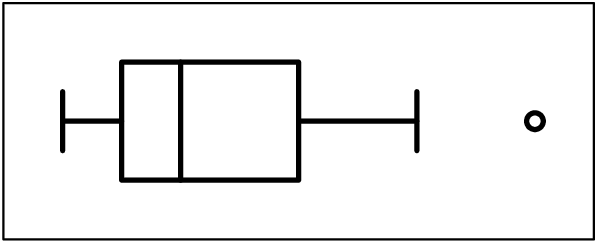
\includegraphics[width=.5\linewidth]{boxplot.png}
\end{figure}

\begin{itemize}
    \item Середня лінія -- медіана.
    \item Ліва границя -- нижній квартиль.
    \item Права границя -- верхній квартиль.
    \item Лівий вус -- найменше значення у вибірці.
    \item Правий вус -- найбільше значення у вибірці.
    \item Викиди позначаються як окремі точки поза вусами.
\end{itemize}

\textbf{Вступ до кореляційного аналізу} \\

Кореляційний аналіз дозволяє з'ясувати питання наявності зв'язку між процесами (явищами, об'єктами) які досліджуються. Для цього, враховуючи тип даних які обробляються, як правило, здійснюють такі кроки: 
\begin{itemize}
    \item Обирають конкретну числову характеристику для парного чи множинного статистичного зв'язку.
    \item Визначають оцінку значення цієї характеристики.
    \item На основі цієї оцінки приймають рішення, чи є істинним зв'язок що досліджується.
\end{itemize}

Тільки після отримання стверджувальної відповіді щодо істинності статистичного зв'язку між змінними має сенс переходити до пошуку математичної моделі цього зв'язку. \\

\textbf{Додаток: умовні ймовірності та математчині сподівання} \\

Нехай $d_\RR$ є сім'єю усіх напівінтервалів вигляду $(a, b]$, $a, b \in \RR$. Борелівською $\sigma$-алгеброю $\sigma_\RR$ в $\RR$ називається найменша $\sigma$-алгебра яка містить у собі сім'ю $d_\RR$. Борелівська $\sigma$-алгебра $\sigma_{\RR^q}$ в $\RR^q$ визначається аналогічно (на напіввідкритих брусах). \\

\textbf{Зауваження.} З визначення борелівської $\sigma$-алгебри $\sigma_\RR$ в $\RR$ випливає, що у неї, окрім згаданих півінтервалів входять також інтервали, сегменти і півінтервали $[a, b)$, причому всі з кінцями із $\bar{\RR} = \RR \cup \{ -\infty, \infty \}$, причому кожну із цих сімей (інтервалів, відрізків, тощо) можна використовувати у визначенні замість вищезгаданих півінтервалів. \\

Борелівською множиною в $\RR$ (множиною, вимірною за Борелем в $\RR$) називається довільна множина із Борелівської $\sigma$-алгебри $\sigma_\RR$ в $\RR$. Борелівська множина в $\RR^q$ (множина, вимірна за Борелем в $\RR^q$) визначається аналогічно.\\

Борелівською функцією в $\RR$ (функцією, вимірною за Борелем в $\RR$) називається дійсна функція для якої прообраз довільної борелівської множини в $\RR$ є борелівською множиною в $\RR$. Борелівська функція з областю визначення у просторі $\RR^q$ визначається аналогічно. \\

Нехай на ймовірнісному просторі $(\Omega, F, P)$ задані дійсні випадкові величини $\eta = \eta(\omega)$ та $\xi = \xi(\omega)$, а $G$ -- деяка $\sigma$-алгебра з $F$. Випадкова величина $\xi$ називається вимірною відносно $G$ якщо прообраз довільної борелівської множини в $\RR$ належить $G$. \\

Умовним математчиним сподіванням невід'ємної випадкової величини $\xi$ відносно $G$ називається невід'ємна випадкова величина яка позначається $M(\xi / G)$ або $M(\xi / G)(\omega)$ така, що:
\begin{itemize}
    \item $M(\xi / G)$ є вимірною відносно $G$;
    \item $\forall A \in G: \int_A \xi \diff P = \int_A M(\xi / G) \diff P$.
\end{itemize}

Нескладно з'ясувати питання існування та єдиності $M(\xi / G)$. \\

Справді, якщо випадкова величина є інтегровню і $\xi \ge 0$ майже всюди, то на вимірному просторі $(\Omega, G)$ функція множини $\lambda(A) = \int_A \xi \diff P$ є скінченною, $\sigma$-адитивною, і абсолютно неперервною відносно ймовірносної міри $P$ мірою.

\begin{theorem}[Радана-Никодима]
    Нехай $(\Omega, \sigma_\Omega)$ -- вимірний простір, на $\sigma_\Omega$ задано скінченні та $\sigma$-адитивні міри $\lambda$ та $\mu$. Якщо $\lambda$ є абсолютно неперервною відносно $\mu$, то існує єдина з точністю до $\mu$-еквівалентності $\sigma_\Omega$-вимірна функція $\phi(\cdot)$ на $\Omega$ яка задовольняє наступним вимогам:
    \begin{itemize}
        \item $\phi \in L_1(\Omega, \sigma_\Omega, \mu)$, тобто $\phi$ інтегровна на $\Omega$ за $\mu$;
        \item $\phi(\omega) \ge 0$ майже всюди на $\Omega$ відносно $\mu$;
        \item $\lambda(A) = \int_A \phi \diff \mu$
    \end{itemize}
\end{theorem}

З цієї теоерми випливає, що існує єдина з точністю до $P$-еквівалентності невід'ємна інтегровна $G$-вимірна функція $M(\xi / G)$ на $\Omega$ така, що \[ \lambda(A) = \Int_A \xi \diff P = \Int_A M(\xi / G) \diff P, \quad \forall A \in G. \]

Отже для невід'ємно випадкової величини $\xi$ існує єдине з точністю до $P$-еквівалентності умовне математичне сподівання відносно $G$, а саме $M(\xi / G)$. \\

Для знакових математичних величин $\xi$ умовне математичне сподівання вводитсья як $M(\xi / G) = M(\xi^+ / G) - M(\xi^- / G)$, де $\xi^+ = \max(\xi, 0)$, $\xi^- = - \min(\xi, 0)$. Зрозуміло що воно визначене коректно тоді і тільки тоді, коли хоча б одне з $ M(\xi^+ / G)$, $M(\xi^- / G)$ скінченне. \\

Умовна ймовірність події $B \in F$ визначається як умовне математичне сподівання індикаторної функції цієї події. Зауважимо, що її також можна задати через її властивість: \[ P(A \cup B) = \Int_A P(B / G) \diff P. \] 

\end{document}
